\documentclass[10pt,a4paper]{article}
\usepackage[landscape,margin=15mm]{geometry}
\usepackage{newtxtext,newtxmath,graphicx,booktabs,array}
\usepackage[hidelinks]{hyperref}
\hypersetup{pdftitle={LogicConnect Evidence Atlas},pdfauthor={}}
\begin{document}
\section*{LogicConnect: Evidence Atlas}
Detailed supporting results and plots for internal review and presentation. This artifact is separate from the DATE submission. LC denotes the unified construction; LC-D is a distinct dense specialization. All local values come from the frozen evidence snapshot. Reported literature values retain separate labels and source records. No new training or inference was performed.
\clearpage
\section*{Dense held-out accuracy: all methods and seeds}
T throughout; three seeds. LogicConnect-D is the distinct dense specialization. A best-of-variants test maximum is not an evaluated method-selection policy.
\par\bigskip
\setlength{\tabcolsep}{2pt}
\begin{tabular}{@{}p{57mm}p{37.0mm}p{37.0mm}p{37.0mm}p{37.0mm}p{37.0mm}@{}}
\toprule
Model & Gates & Method & Mean $\pm$ SD (\%) & Seeds 0, 1, 2 (\%) & Source \\ \midrule
MNIST & 8000 & Random & 91.273 $\pm$ 0.217 & 91.190, 91.520, 91.110 & REP \\
MNIST & 8000 & LogicConnect & 91.937 $\pm$ 0.137 & 91.790, 91.960, 92.060 & OUR \\
MNIST & 8000 & LogicConnect-D & 91.907 $\pm$ 0.307 & 91.570, 91.980, 92.170 & OUR \\
Fashion-MNIST & 16000 & Random & 85.197 $\pm$ 0.261 & 85.110, 85.490, 84.990 & REP \\
Fashion-MNIST & 16000 & LogicConnect & 85.717 $\pm$ 0.453 & 85.340, 85.590, 86.220 & OUR \\
Fashion-MNIST & 16000 & LogicConnect-D & 85.913 $\pm$ 0.356 & 86.280, 85.890, 85.570 & OUR \\
CIFAR-10 S & 48000 & Random & 48.913 $\pm$ 0.346 & 48.840, 49.290, 48.610 & REP \\
CIFAR-10 S & 48000 & LogicConnect & 52.097 $\pm$ 0.630 & 52.070, 51.480, 52.740 & OUR \\
CIFAR-10 S & 48000 & LogicConnect-D & 52.390 $\pm$ 0.295 & 52.400, 52.680, 52.090 & OUR \\
CIFAR-10 M & 512000 & Random & 54.097 $\pm$ 0.171 & 53.900, 54.210, 54.180 & REP \\
\bottomrule
\end{tabular}
\clearpage
\section*{Dense held-out accuracy: all methods and seeds (continued)}
\setlength{\tabcolsep}{2pt}
\begin{tabular}{@{}p{57mm}p{37.0mm}p{37.0mm}p{37.0mm}p{37.0mm}p{37.0mm}@{}}
\toprule
Model & Gates & Method & Mean $\pm$ SD (\%) & Seeds 0, 1, 2 (\%) & Source \\ \midrule
CIFAR-10 M & 512000 & LogicConnect & 58.653 $\pm$ 0.168 & 58.800, 58.690, 58.470 & OUR \\
CIFAR-10 M & 512000 & LogicConnect-D & 58.357 $\pm$ 0.253 & 58.450, 58.070, 58.550 & OUR \\
CIFAR-10 L & 1280000 & Random & 55.870 $\pm$ 0.308 & 55.820, 55.590, 56.200 & REP \\
CIFAR-10 L & 1280000 & LogicConnect & 60.463 $\pm$ 0.348 & 60.080, 60.550, 60.760 & OUR \\
CIFAR-10 L & 1280000 & LogicConnect-D & 61.073 $\pm$ 0.463 & 60.540, 61.310, 61.370 & OUR \\
\bottomrule
\end{tabular}
\clearpage
\section*{Dense paired effects against native random}
T, paired over the complete three-seed set. Intervals are not adjusted for multiple comparisons. Both variants are retained.
\par\bigskip
\setlength{\tabcolsep}{2pt}
\begin{tabular}{@{}p{57mm}p{37.0mm}p{37.0mm}p{37.0mm}p{37.0mm}p{37.0mm}@{}}
\toprule
Model & Method & Gain (pp) & Paired 95\% CI & Wins / 3 & Raw gains (pp) \\ \midrule
MNIST & LogicConnect & 0.663 & [0.015, 1.311] & 3 & 0.600, 0.440, 0.950 \\
MNIST & LogicConnect-D & 0.633 & [-0.290, 1.557] & 3 & 0.380, 0.460, 1.060 \\
Fashion-MNIST & LogicConnect & 0.520 & [-1.016, 2.056] & 3 & 0.230, 0.100, 1.230 \\
Fashion-MNIST & LogicConnect-D & 0.717 & [-0.284, 1.717] & 3 & 1.170, 0.400, 0.580 \\
CIFAR-10 S & LogicConnect & 3.183 & [0.772, 5.595] & 3 & 3.230, 2.190, 4.130 \\
CIFAR-10 S & LogicConnect-D & 3.477 & [3.265, 3.688] & 3 & 3.560, 3.390, 3.480 \\
CIFAR-10 M & LogicConnect & 4.557 & [3.781, 5.332] & 3 & 4.900, 4.480, 4.290 \\
CIFAR-10 M & LogicConnect-D & 4.260 & [3.371, 5.149] & 3 & 4.550, 3.860, 4.370 \\
CIFAR-10 L & LogicConnect & 4.593 & [3.721, 5.466] & 3 & 4.260, 4.960, 4.560 \\
CIFAR-10 L & LogicConnect-D & 5.203 & [3.959, 6.447] & 3 & 4.720, 5.720, 5.170 \\
\bottomrule
\end{tabular}
\clearpage
\section*{Convolutional accuracy and training cost}
S/M are nine-channel, paper-faithful architectures. V and T are separate observations. Recorded wall times include evaluation and depend on execution conditions. GPU is peak PyTorch allocation.
\par\bigskip
\setlength{\tabcolsep}{2pt}
\begin{tabular}{@{}p{29mm}p{29.6mm}p{29.6mm}p{29.6mm}p{29.6mm}p{29.6mm}p{29.6mm}p{29.6mm}@{}}
\toprule
Size & Method & Scope & n & Accuracy (\%) & Time (h) & GPU (GiB) & Gate functions \\ \midrule
S & Random & T & 1 & 57.370 & 4.975 & 1.831 & 83552 \\
S & LogicConnect & T & 1 & 60.630 & 4.951 & 1.831 & 83552 \\
M & Random & T & 1 & 69.570 & 25.470 & 14.614 & 668416 \\
M & LogicConnect & T & 1 & 71.650 & 35.686 & 14.614 & 668416 \\
S & Random & V & 3 & 59.820 $\pm$ 1.130 & 4.966 & 1.831 & 83552 \\
S & LogicConnect & V & 3 & 61.053 $\pm$ 1.041 & 4.970 & 1.831 & 83552 \\
\bottomrule
\end{tabular}
\clearpage
\section*{LILogic architectures: achieved and reported values}
LILogic v2 (2026), seven thresholds. Published time is contextual because execution platforms and implementations differ. Reported peak GPU allocation is unavailable. Top-32 local n=1; fixed methods n=3.
\par\bigskip
\setlength{\tabcolsep}{2pt}
\begin{tabular}{@{}p{29mm}p{25.5mm}p{25.5mm}p{25.5mm}p{25.5mm}p{25.5mm}p{25.5mm}p{25.5mm}p{25.5mm}@{}}
\toprule
Size & Method & n & Local T (\%) & Local min & Local GiB & Params (M) & Reported T (\%) & Reported min \\ \midrule
M & Random & 3 & 49.010 $\pm$ 0.426 & 14.622 & 0.474 & 1.024 & 49.17 $\pm$ 0.14 & 2.9 \\
M & LogicConnect & 3 & 52.543 $\pm$ 0.296 & 14.593 & 0.474 & 1.024 & -- & -- \\
M & Top-32 & 1 & 57.840 & 37.808 & 8.100 & 5.120 & 57.28 $\pm$ 0.30 & 15.3 \\
L & Random & 3 & 55.333 $\pm$ 0.469 & 15.202 & 1.557 & 4.096 & 54.76 $\pm$ 0.27 & 16.3 \\
L & LogicConnect & 3 & 60.193 $\pm$ 0.286 & 18.472 & 1.557 & 4.096 & -- & -- \\
L & Top-32 & 1 & 62.030 & 350.635 & 24.861 & 20.480 & 60.98 $\pm$ 0.19 & 297.2 \\
\bottomrule
\end{tabular}
\clearpage
\section*{Derived routing trade-offs}
Ratios use locally observed means. These quantities describe an accuracy/resource trade-off, not a claim of universal dominance or a controlled timing speedup.
\par\bigskip
\setlength{\tabcolsep}{2pt}
\begin{tabular}{@{}p{29mm}p{35.0mm}p{35.0mm}p{35.0mm}p{35.0mm}p{35.0mm}p{35.0mm}@{}}
\toprule
Size & Accuracy cost (pp) & Top-32 / LC GPU & GPU saved (\%) & Observed time ratio & Params saved (\%) & Top-32 gain recovered (\%) \\ \midrule
M & 5.297 & 17.103 & 94.153 & 2.591 & 80.000 & 40.015 \\
L & 1.837 & 15.967 & 93.737 & 18.982 & 80.000 & 72.573 \\
\bottomrule
\end{tabular}
\clearpage
\section*{Unified dense construction overhead}
All rows use the unified constructor; no dense-specialization construction times are substituted. Training includes evaluation.
\par\bigskip
\setlength{\tabcolsep}{2pt}
\begin{tabular}{@{}p{57mm}p{47.0mm}p{47.0mm}p{47.0mm}p{47.0mm}@{}}
\toprule
Model & CPU construction (s) & Training (min) & GPU (GiB) & Construction / training (\%) \\ \midrule
MNIST & 0.100 & 14.623 & 0.017 & 0.011 \\
Fashion-MNIST & 0.231 & 14.594 & 0.034 & 0.026 \\
CIFAR-10 S & 0.916 & 12.115 & 0.106 & 0.126 \\
CIFAR-10 M & 14.333 & 41.389 & 1.123 & 0.577 \\
CIFAR-10 L & 31.218 & 113.526 & 2.717 & 0.458 \\
\bottomrule
\end{tabular}
\clearpage
\section*{Dense first/deeper factorial: complete seed table}
V, dense M at 20K updates. S retains LogicConnect; R preserves each predecessor degree in each input slot while randomizing pair identities. Native random is not the RR control.
\par\bigskip
\setlength{\tabcolsep}{2pt}
\begin{tabular}{@{}p{57mm}p{47.0mm}p{47.0mm}p{47.0mm}p{47.0mm}@{}}
\toprule
Arm & Mean $\pm$ SD (\%) & Seeds 0, 1, 2 (\%) & Time (min) & GPU (GiB) \\ \midrule
SS & 59.133 $\pm$ 0.316 & 58.860, 59.480, 59.060 & 7.754 & 1.123 \\
SR & 58.613 $\pm$ 0.324 & 58.820, 58.780, 58.240 & 7.705 & 1.123 \\
RS & 54.640 $\pm$ 0.541 & 54.260, 55.260, 54.400 & 7.743 & 1.123 \\
RR & 54.927 $\pm$ 0.522 & 54.800, 54.480, 55.500 & 7.779 & 1.123 \\
\bottomrule
\end{tabular}
\clearpage
\section*{Dense factorial: all five contrasts}
V, exploratory and unadjusted. First-layer effects have positive intervals. The additional deeper effect and interaction remain inconclusive.
\par\bigskip
\setlength{\tabcolsep}{2pt}
\begin{tabular}{@{}p{57mm}p{47.0mm}p{47.0mm}p{47.0mm}p{47.0mm}@{}}
\toprule
Contrast & Gain (pp) & Paired 95\% CI & Wins / 3 & Raw gains (pp) \\ \midrule
deeper given randomized first & -0.287 & [-2.685, 2.111] & 1 & -0.540, 0.780, -1.100 \\
deeper given structured first & 0.520 & [-0.523, 1.563] & 3 & 0.040, 0.700, 0.820 \\
first given randomized deeper & 3.687 & [1.621, 5.753] & 3 & 4.020, 4.300, 2.740 \\
first given structured deeper & 4.493 & [3.901, 5.086] & 3 & 4.600, 4.220, 4.660 \\
interaction & 0.807 & [-1.725, 3.338] & 2 & 0.580, -0.080, 1.920 \\
\bottomrule
\end{tabular}
\clearpage
\section*{Dense M stage-selection controls}
V, exploratory. The body/classifier effects condition on a fixed reference-ancestry classifier. WARP is an adapted recipe and trails the matched raw representation. These controls do not establish an isolated benefit from ancestry scoring.
\par\bigskip
\setlength{\tabcolsep}{2pt}
\begin{tabular}{@{}p{57mm}p{47.0mm}p{47.0mm}p{47.0mm}p{47.0mm}@{}}
\toprule
Comparison & Gain (pp) & Paired 95\% CI & n & Wins \\ \midrule
LC minus random & 4.313 & [2.475, 6.152] & 3 & 3 \\
LC minus balanced random & 0.487 & [-0.795, 1.768] & 3 & 3 \\
LC minus nominal & -0.087 & [-1.759, 1.585] & 3 & 1 \\
\bottomrule
\end{tabular}
\clearpage
\section*{Convolutional S stage-selection controls}
V, exploratory. The body/classifier effects condition on a fixed reference-ancestry classifier. WARP is an adapted recipe and trails the matched raw representation. These controls do not establish an isolated benefit from ancestry scoring.
\par\bigskip
\setlength{\tabcolsep}{2pt}
\begin{tabular}{@{}p{57mm}p{47.0mm}p{47.0mm}p{47.0mm}p{47.0mm}@{}}
\toprule
Comparison & Gain (pp) & Paired 95\% CI & n & Wins \\ \midrule
LC minus random & 1.707 & [-2.600, 6.013] & 3 & 3 \\
LC minus balanced random & 0.213 & [-0.836, 1.263] & 3 & 2 \\
LC minus nominal & 0.593 & [-1.121, 2.308] & 3 & 2 \\
\bottomrule
\end{tabular}
\clearpage
\section*{Convolutional body/classifier effects}
V, exploratory. The body/classifier effects condition on a fixed reference-ancestry classifier. WARP is an adapted recipe and trails the matched raw representation. These controls do not establish an isolated benefit from ancestry scoring.
\par\bigskip
\setlength{\tabcolsep}{2pt}
\begin{tabular}{@{}p{57mm}p{47.0mm}p{47.0mm}p{47.0mm}p{47.0mm}@{}}
\toprule
Comparison & Gain (pp) & Paired 95\% CI & n & Wins \\ \midrule
body with random head & 1.207 & [-3.169, 5.582] & 3 & 3 \\
body with LC head & 2.140 & [0.674, 3.606] & 3 & 3 \\
head with random body & -0.433 & [-5.725, 4.858] & 3 & 1 \\
head with LC body & 0.500 & [-1.410, 2.410] & 3 & 2 \\
body head interaction & 0.933 & [-4.766, 6.633] & 3 & 2 \\
\bottomrule
\end{tabular}
\clearpage
\section*{Dense M adapted-WARP effect}
V, exploratory. The body/classifier effects condition on a fixed reference-ancestry classifier. WARP is an adapted recipe and trails the matched raw representation. These controls do not establish an isolated benefit from ancestry scoring.
\par\bigskip
\setlength{\tabcolsep}{2pt}
\begin{tabular}{@{}p{57mm}p{47.0mm}p{47.0mm}p{47.0mm}p{47.0mm}@{}}
\toprule
Comparison & Gain (pp) & Paired 95\% CI & n & Wins \\ \midrule
LC minus random & 4.700 & [3.919, 5.481] & 3 & 3 \\
\bottomrule
\end{tabular}
\clearpage
\section*{Convolutional S adapted-WARP effect}
V, exploratory. The body/classifier effects condition on a fixed reference-ancestry classifier. WARP is an adapted recipe and trails the matched raw representation. These controls do not establish an isolated benefit from ancestry scoring.
\par\bigskip
\setlength{\tabcolsep}{2pt}
\begin{tabular}{@{}p{57mm}p{47.0mm}p{47.0mm}p{47.0mm}p{47.0mm}@{}}
\toprule
Comparison & Gain (pp) & Paired 95\% CI & n & Wins \\ \midrule
LC minus random & 0.087 & [-1.243, 1.417] & 3 & 1 \\
\bottomrule
\end{tabular}
\clearpage
\section*{Frozen CIFAR-10.1 transfer}
T, no adaptation. One-time frozen evaluation. Single-seed convolutional points have no across-seed interval.
\par\bigskip
\setlength{\tabcolsep}{2pt}
\begin{tabular}{@{}p{57mm}p{47.0mm}p{47.0mm}p{47.0mm}p{47.0mm}@{}}
\toprule
Model & LC gain (pp) & Paired 95\% CI & n & Wins \\ \midrule
dense\_m & 3.733 & [2.801, 4.666] & 3 & 3 \\
conv\_s & -0.050 & -- & 1 & 0 \\
conv\_m & 1.950 & -- & 1 & 1 \\
\bottomrule
\end{tabular}
\clearpage
\section*{Third-round inventory, including negative reproductions}
The BitLogic-related local reproductions failed to reproduce the published accuracy. They are preserved as negative evidence; low local comparator accuracy is not evidence of superiority over published BitLogic. Rank and protocol differences prevent topology-only attribution across arbitrary rows.
\par\bigskip
\setlength{\tabcolsep}{2pt}
\begin{tabular}{@{}p{29mm}p{25.5mm}p{25.5mm}p{25.5mm}p{25.5mm}p{25.5mm}p{25.5mm}p{25.5mm}p{25.5mm}@{}}
\toprule
Protocol & Size & Method & Rank & n & Local T (\%) & Time (min) & GPU (GiB) & Provenance \\ \midrule
BitLogic-adapted & L & Learned rank-4 & 4 & 2 & 13.160 $\pm$ 0.240 & 164.470 & 9.456 & reproduced-local \\
BitLogic-adapted & L & Random & 2 & 2 & 25.160 $\pm$ 0.156 & 8.520 & 0.414 & reproduced-local \\
BitLogic-adapted & L & LogicConnect & 2 & 2 & 25.930 $\pm$ 2.871 & 8.561 & 0.414 & our-transfer \\
BitLogic-adapted & M & Learned rank-4 & 4 & 2 & 16.625 $\pm$ 0.078 & 41.206 & 2.372 & reproduced-local \\
BitLogic-adapted & M & Random & 2 & 2 & 25.945 $\pm$ 0.870 & 8.582 & 0.104 & reproduced-local \\
BitLogic-adapted & M & LogicConnect & 2 & 2 & 26.040 $\pm$ 0.014 & 8.644 & 0.104 & our-transfer \\
BitLogic-adapted & S & Learned rank-4 & 4 & 2 & 27.500 $\pm$ 0.113 & 9.921 & 0.611 & reproduced-local \\
BitLogic-adapted & S & Random & 2 & 2 & 26.175 $\pm$ 0.445 & 8.499 & 0.028 & reproduced-local \\
BitLogic-adapted & S & LogicConnect & 2 & 2 & 28.435 $\pm$ 1.648 & 8.472 & 0.028 & our-transfer \\
LILogic & L & Random & 2 & 3 & 55.333 $\pm$ 0.469 & 15.202 & 1.557 & reproduced-local \\
\bottomrule
\end{tabular}
\clearpage
\section*{Third-round inventory, including negative reproductions (continued)}
\setlength{\tabcolsep}{2pt}
\begin{tabular}{@{}p{29mm}p{25.5mm}p{25.5mm}p{25.5mm}p{25.5mm}p{25.5mm}p{25.5mm}p{25.5mm}p{25.5mm}@{}}
\toprule
Protocol & Size & Method & Rank & n & Local T (\%) & Time (min) & GPU (GiB) & Provenance \\ \midrule
LILogic & L & Top-32 & 2 & 1 & 62.030 & 350.635 & 24.861 & reproduced-local \\
LILogic & L & LogicConnect & 2 & 3 & 60.193 $\pm$ 0.286 & 18.472 & 1.557 & our-transfer \\
LILogic & M & Random & 2 & 3 & 49.010 $\pm$ 0.426 & 14.622 & 0.474 & reproduced-local \\
LILogic & M & Top-32 & 2 & 1 & 57.840 & 37.808 & 8.100 & reproduced-local \\
LILogic & M & LogicConnect & 2 & 3 & 52.543 $\pm$ 0.296 & 14.593 & 0.474 & our-transfer \\
Original dense & L & LogicConnect & 2 & 3 & 60.463 $\pm$ 0.348 & 113.526 & 2.717 & our-transfer \\
Original dense & M & LogicConnect & 2 & 3 & 58.653 $\pm$ 0.168 & 41.389 & 1.123 & our-transfer \\
\bottomrule
\end{tabular}
\clearpage
\section*{Dense Results}
\begin{center}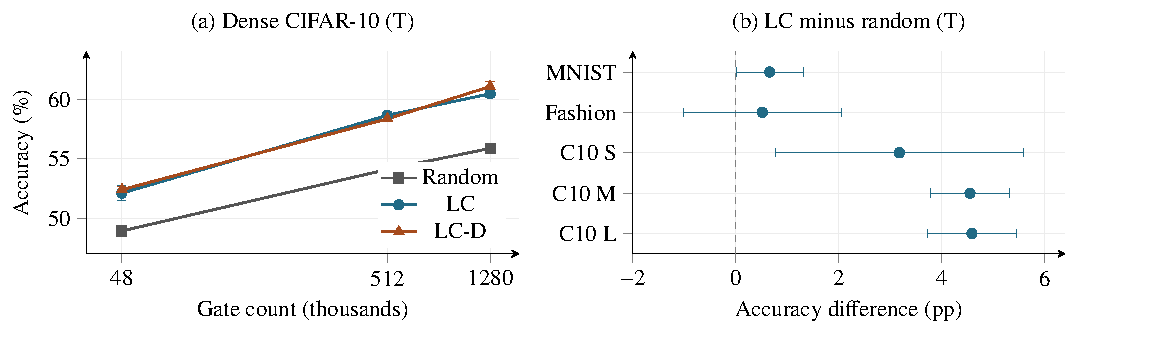
\includegraphics[width=184mm]{figures/dense_results_plot.pdf}\end{center}
Dense accuracy at fixed budgets. (a) Mean $\pm$ sample SD over three seeds. LC-D is the separate dense specialization. (b) Paired 95\% confidence intervals for LC minus random; all three CIFAR-10 intervals exclude zero.
\clearpage
\section*{Routing Tradeoff}
\begin{center}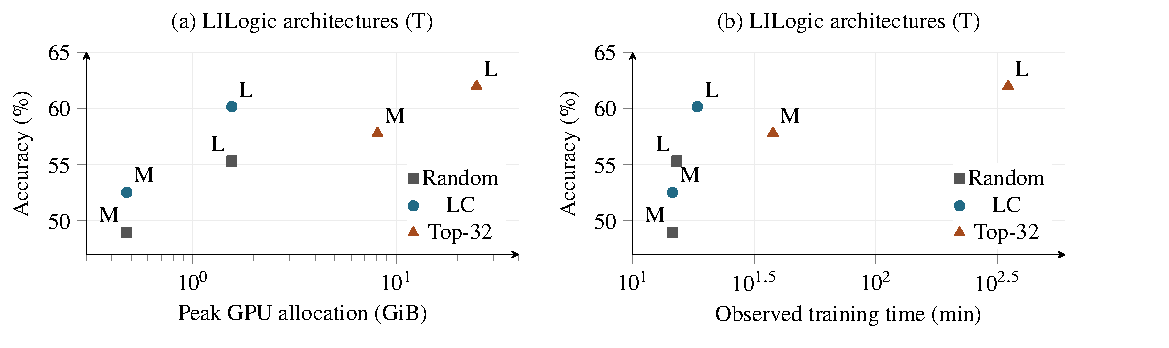
\includegraphics[width=184mm]{figures/routing_tradeoff_plot.pdf}\end{center}
Accuracy versus (a) peak GPU allocation and (b) observed training time under the LILogic M/L configurations. LC and random: three seeds, mean $\pm$ sample SD. Top-32: one seed. M/L identify architectures; wall-time ratios are descriptive execution measurements.
\clearpage
\section*{Structural Ablation}
\begin{center}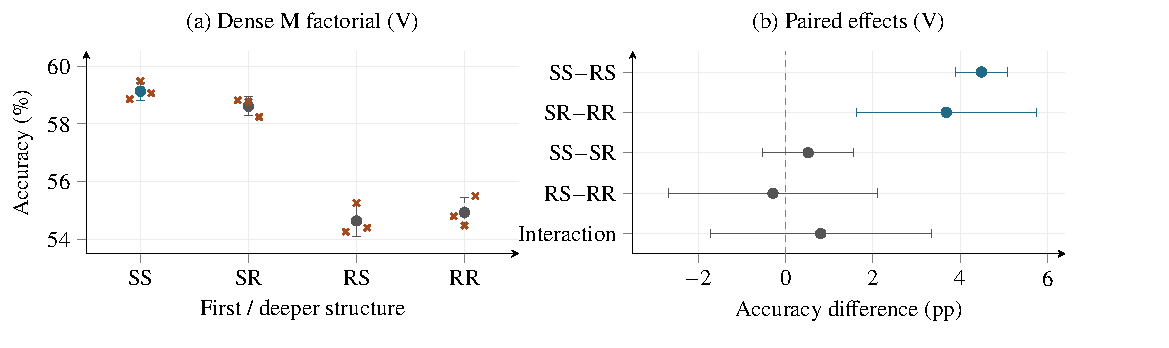
\includegraphics[width=184mm]{figures/structural_ablation_plot.pdf}\end{center}
Dense M attribution at 20K updates. S retains LC structure; R randomizes pairs while preserving each predecessor degree in each input slot. (a) Three seed values (crosses) and mean $\pm$ sample SD. (b) All five paired 95\% intervals, exploratory and unadjusted. The first two contrasts isolate first-layer structure.
\clearpage
\section*{Conv Replication}
\begin{center}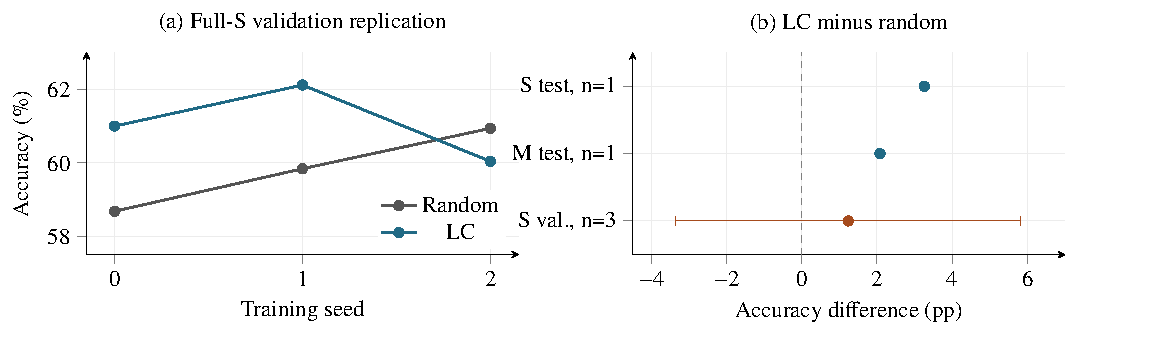
\includegraphics[width=184mm]{figures/conv_replication_plot.pdf}\end{center}
Convolutional replication and measurement scope. Single-seed tests have no error bars. Full-S validation uses three paired seeds with a 95\% interval; its third seed reverses the sign of the gain. Validation and test observations are not pooled.
\clearpage
\section*{Construction Cost}
\begin{center}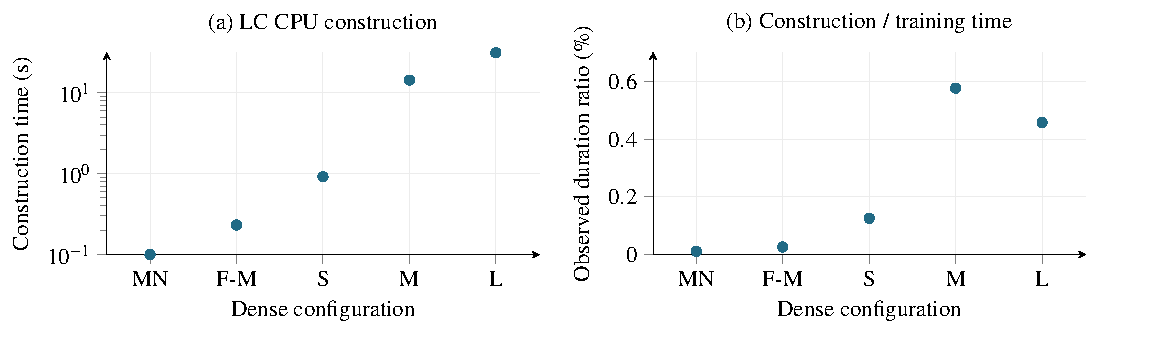
\includegraphics[width=184mm]{figures/construction_cost_plot.pdf}\end{center}
Offline LC construction for MNIST (MN), Fashion-MNIST (F-M), and CIFAR-10 S/M/L. Ratios use recorded training duration, including evaluation; they do not measure a controlled end-to-end speedup.
\clearpage
\section*{Mechanism Controls}
\begin{center}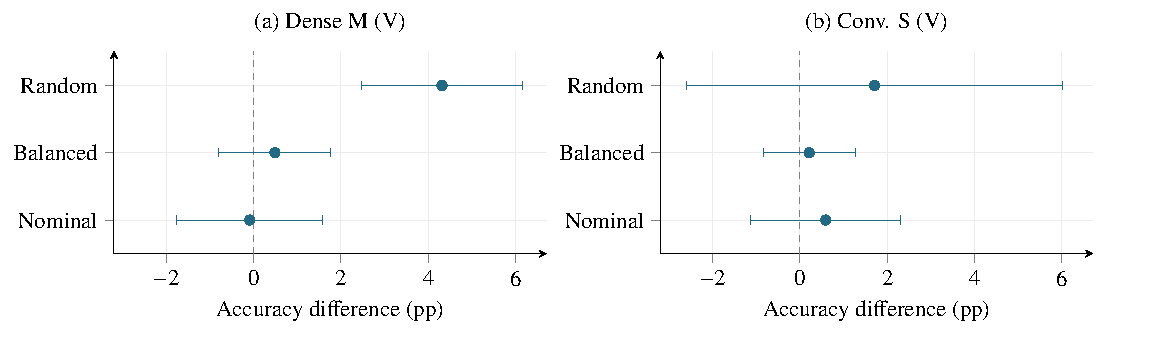
\includegraphics[width=184mm]{figures/mechanism_controls_plot.pdf}\end{center}
LC minus each stage-selection control at 20K updates, three paired seeds and exploratory 95\% intervals. Neither coordinate establishes an incremental benefit over the nominal schedule. The balanced control is distinct from native random wiring.
\clearpage
\section*{Conv Factorial}
\begin{center}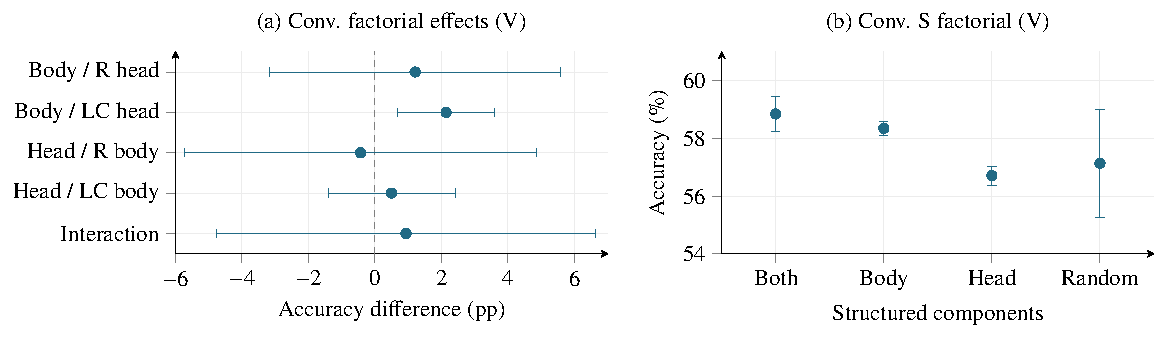
\includegraphics[width=184mm]{figures/conv_factorial_plot.pdf}\end{center}
Convolutional body/classifier attribution at 20K updates, three seeds. The structured classifier retains reference-body ancestry, so body effects are conditional on that classifier. (a) All five exploratory paired 95\% intervals. (b) Mean $\pm$ sample SD.
\clearpage
\section*{Warp Compatibility}
\begin{center}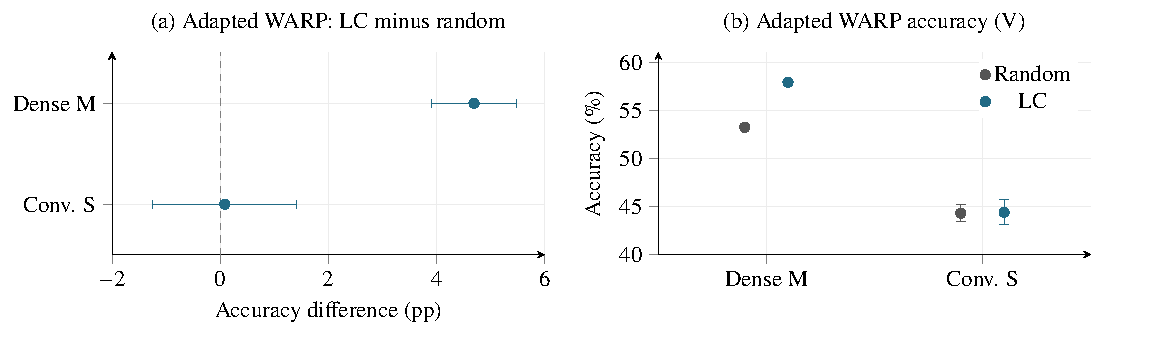
\includegraphics[width=184mm]{figures/warp_compatibility_plot.pdf}\end{center}
Compatibility with adapted WARP training. Dense M uses 108K updates; convolutional S uses 20K. Three seeds; paired 95\% intervals in (a), mean $\pm$ sample SD in (b). Both adapted recipes trail matched raw training; these data do not reproduce WARP\textquotesingle s published headline results.
\clearpage
\section*{Transfer}
\begin{center}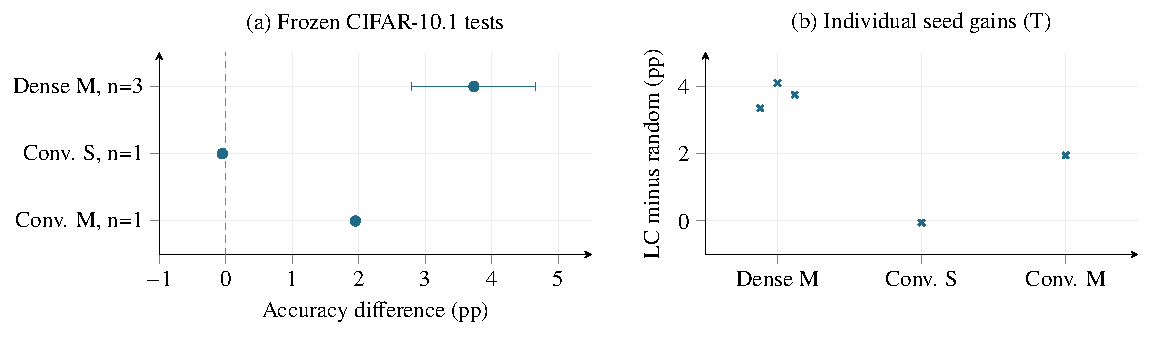
\includegraphics[width=184mm]{figures/transfer_plot.pdf}\end{center}
Frozen CIFAR-10.1 evaluation without adaptation or repeat inference. Dense M has a three-seed paired 95\% interval; convolutional points each use one seed. (b) All available paired seed differences.
\clearpage
\section*{Dense Seed Gains}
\begin{center}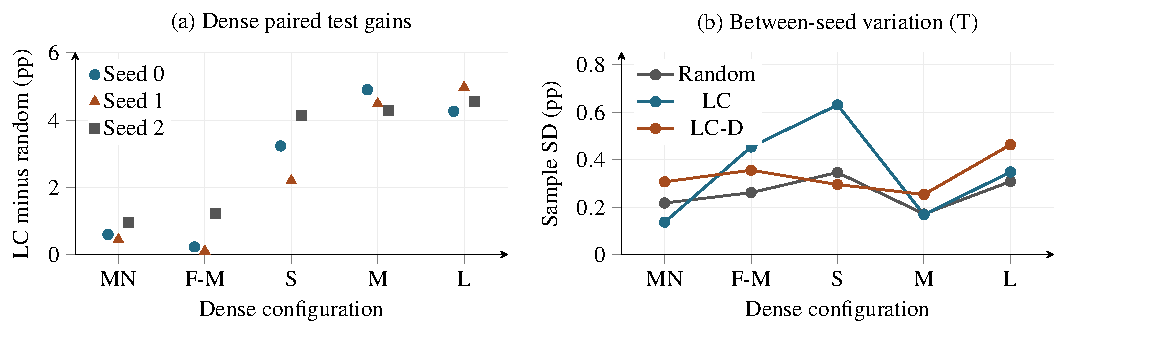
\includegraphics[width=184mm]{figures/dense_seed_gains_plot.pdf}\end{center}
All 15 paired dense LC test differences and the sample standard deviations of all three fixed constructions. MN/F-M denote MNIST/Fashion-MNIST; S/M/L denote CIFAR-10 sizes. Positive seed differences do not guarantee that every three-seed confidence interval excludes zero.
\end{document}
